% !TEX TS-program = pdflatex
% !TEX encoding = UTF-8 Unicode

% This is a simple template for a LaTeX document using the "article" class.
% See "book", "report", "letter" for other types of document.

\documentclass[11pt]{book} % use larger type; default would be 10pt

\usepackage[utf8]{inputenc} % set input encoding (not needed with XeLaTeX)
\usepackage{hyperref}
\usepackage{amsmath,amsthm}
\usepackage{pgf,tikz}
\usetikzlibrary{arrows}

%%% Examples of Article customizations
% These packages are optional, depending whether you want the features they provide.
% See the LaTeX Companion or other references for full information.

%%% PAGE DIMENSIONS
\usepackage{geometry} % to change the page dimensions
\geometry{a4paper} % or letterpaper (US) or a5paper or....
% \geometry{margin=2in} % for example, change the margins to 2 inches all round
% \geometry{landscape} % set up the page for landscape
%   read geometry.pdf for detailed page layout information

\usepackage{graphicx} % support the \includegraphics command and options

% \usepackage[parfill]{parskip} % Activate to begin paragraphs with an empty line rather than an indent

%%% PACKAGES
\usepackage{booktabs} % for much better looking tables
\usepackage{array} % for better arrays (eg matrices) in maths
\usepackage{paralist} % very flexible & customisable lists (eg. enumerate/itemize, etc.)
\usepackage{verbatim} % adds environment for commenting out blocks of text & for better verbatim
\usepackage{subfig} % make it possible to include more than one captioned figure/table in a single float
% These packages are all incorporated in the memoir class to one degree or another...

\usepackage{exercise}
\renewcounter{Exercise}[section]% Reset counter every chapter
\renewcommand{\theExercise}{\thesection.\arabic{Exercise}}%


%%% HEADERS & FOOTERS
\usepackage{fancyhdr} % This should be set AFTER setting up the page geometry
\pagestyle{fancy} % options: empty , plain , fancy
\renewcommand{\headrulewidth}{0pt} % customise the layout...
\lhead{}\chead{}\rhead{}
\lfoot{}\cfoot{\thepage}\rfoot{}

%%% SECTION TITLE APPEARANCE
\usepackage{sectsty}
\allsectionsfont{\sffamily\mdseries\upshape} % (See the fntguide.pdf for font help)
% (This matches ConTeXt defaults)

%%% ToC (table of contents) APPEARANCE
\usepackage[nottoc,notlof,notlot]{tocbibind} % Put the bibliography in the ToC
\usepackage[titles,subfigure]{tocloft} % Alter the style of the Table of Contents
\renewcommand{\cftsecfont}{\rmfamily\mdseries\upshape}
\renewcommand{\cftsecpagefont}{\rmfamily\mdseries\upshape} % No bold!

%%% END Article customizations

%%% The "real" document content comes below...

\title{Larson's Solutions}
\author{Shuai Jiang}
%\date{} % Activate to display a given date or no date (if empty),
         % otherwise the current date is printed 

\begin{document}
\maketitle
\tableofcontents

\chapter*{Preface}
\begin{itemize}
	\item This is an attempt at putting together a thorough solution guide to Larson's book. 
	\item Although I dabbled in mathematics all my life, I believe my proof-writing skills are still weak. Please contact me about suggestions and errors! 
\end{itemize}

\chapter{Heuristics}
\section{Search for a Pattern}
\setcounter{Exercise}{5}
\begin{Exercise}
We just have to show that there exists an infinite number of the digit 6 in the sequence, and not to find a closed-form expression of it. If we extend the sequence, it should be of the following form $2,7,1,4,7,4,2,8,2,8,8,1,6,1,6,1,6,6,4,8,6,6,6,6,\ldots$ 

The 4 consecutive 6's seems intriguing, so lets study what happens when we expand it out according to our rule: $3,6,3,6,3,6,3,6$. 
This is good! Four consecutive 6's produces four more 6's, but the next iteration doesn't seem so promising: $1,8,1,8,1,8,1,8,1,8,1,8,1,8$. There are no 6's this time. 

Let's not give up so early, here are the next few iterations (with truncation): 
\begin{align}
8,8,\ldots, 8 \rightarrow 6,4,6,4,\ldots,6,4 \rightarrow 2,4,2,4,\ldots, 2,4 \rightarrow 8,8,\ldots, 8. 
\end{align}
This is great news! We actually found a cycle which gaurentees us more 6's if we follow it, and hence the exercise is proven (informally). \qed
\end{Exercise}

\begin{Exercise}
All prime numbers satisfy the property that the first $n-1$ digit of $S_n$ are $n$. This pattern is fairly obvious if one
starts to extend the $S_n$ sequences out a bit more. The first conjecture might be that all odd numbers satisfy the property,
but the case of $S_9$ is a counter-example. 

The proof is as follows: we first note that if $n$ is in $S_n$, then it will be incremented to $n+1$ in $S_{n+1}$. 
Next, note that if an element of the sequence is a prime number, it can only increment by one if $n$ (of the index $S_n$)
 is the same prime number.

If we put these two facts together, we see that given a prime $p$, the first $p-1$ numbers will increment along with $S_n$ by
the first statement to reach $p$ as $n \rightarrow p$. 
The speed of incrementation might be different, but we really don't care about that by the second statement. 
If an element of the sequence reached $p$ already, then it'll stay at $p$ since no other numbers will divide it.

Note that the $p, p+1, p+2, \ldots$th numbers will be greater than $p$ by the $S_2$. \qed
\end{Exercise}

\begin{Exercise}
The intuition for this problem is quite easy to grasp as the patterns are laid out before our eyes.
I believe the hard part is putting that solution to words. 
There's one thing that I used in proving (albeit less rigorous than I like) this problem, which is that the 
alternate sum of binomial coefficients is 0. This is a commonly used fact, and is quite useful at times. 

Start with $n=3$ for a concrete example. The following sequence is an acceptable solution: 
\begin{align}
	01212123
	\label{eqn:118}
\end{align}
where each digit signifies the index in Pascal's triangle. We start with the null set, then pick any set with one element 
and alternate with subsets of two elements and so on.
The algorithm is a greedy one, and we wish to show it satisfies all the conditions.

Condition one is easy to show, but why are we guaranteed that conditions (ii) and (iii) of the problem is satisfied?
For condition (iii), note that if we simply alternate in the order of the elements, we will always be able to alternate between
a subset of size $m$ and $m+1$. So in our small example, we would add the subset of just element 1, then add element 2, take 
away element 1, add element 3 and so on.

To see that we do indeed use every subset, we need to put our algorithm into numbers. Using our small example again,
we start with the standard Pascal triangle row: 
\begin{align}
	1\| 3 \| 3 \| 1.
\end{align}
This means our sequence needs to have one 0, three 1's, three 2's and one 3 (like in equation~\ref{eqn:118}).
If we alternate between the $\binom{3}{0}$ and $\binom{3}{1}$ we will end up with this:
\begin{align}
	0\| \dot{2} \| 3 \| 1
\end{align}
where the dot indicates the size of the subset of the end of our sequence. 
Alternating between $\binom{3}{1}$ and $\binom{3}{2}$ will result in 
\begin{align}
	0\| 0 \| \dot{0} \| 1.
\end{align}
This configuration means that our sequence's last element is of size 2, and we have one last subset of size 3 to take care of.
At the end, all our numbers will be 0; this is what we want to capture in our proof.

If one continues this pattern in general for all $n$, we will have the following equation
\begin{align}
	{n \choose n} - \left( {n\choose n-1} - \left( {n \choose n-2} - \cdots \left( {n \choose 1} - {n \choose 0} \right) +1 \right) + \cdots +1 \right)
\end{align}
I realize that's a big jump, but try to convince yourself that if you work out the pattern, it's what you see. 
There's really no work left, as that equation simplifies to the alternating sum of binomial coefficients which is 0! 
This proves\footnote{Not that rigorous I suppose} that our algorithm will satisfy all three conditions. \qed
\end{Exercise}

\begin{Exercise}
Two immediate ways to solve this: 
\begin{itemize}
	\item Look at the Pascal triangle in terms of even-odd. You'll quickly notice a pattern that the odd binomial
	coefficients resemble a Sierpinski triangle. It'll be extremely tedious, but I think given enough patience and
	organization one can count them in terms of the pattern.
	\item Note the following pattern starting from row 1: $1,2,2,4,2,4,4,8,2$. Instead of looking at the powers of 2,
	maybe the exponents will give us more insight: $0,1,1,2,1,2,2,3,1$. An \emph{extremely} astute observer will
	note that it's the number of ones in the binary expansion of the row number! For example, row 3 (1,3,3,1) is 11 in 
	binary so the number of odd coefficients is $2^2$ for the number of 1s in the binary representation. 

	I remembered this trick back in high school, so don't fret if you can't figure this out. The theorem which this is based
	on is Lucas' theorem.\footnote{\url{http://en.wikipedia.org/wiki/Lucas'\_theorem}} \qed
\end{itemize}
\end{Exercise}

\begin{Exercise}
	I'm not sure how to cleverly solve this one. My approach was to look at the equations in various mods (i.e. 2, 4, and 8) 
	and see what I can clobber together. I couldn't prove that all such primes are able to be expressed in the forms though.
\end{Exercise}

\begin{Exercise}
	The conjecture should be fairly simple to make; try writing a few terms of the sequence starting with $1/2, 1, 2, -1$. 
	The limit seems to be 1, which is easily proved with a technique that's covered in 7.6.4 as mentioned in the problem. 

	In order to prove this though, one can approach the problem like 1.1.3. We note that $a_2 = \frac{1}{2-a_1}$. 
	Continuing the series:
	\begin{align}
		a_3 &= \frac{1}{2-a_2} = \frac{1}{2 - \frac{1}{2-a_1}} = \frac{2-a_1}{3-2a_1} \\
		a_4 &= \frac{3-2a_1}{4-3a_1} \\
		a_5 &= \frac{4-3a_1}{5-4a_1}
	\end{align}
	The patterns is quite obvious now: 
	\begin{align}
		a_n &= \frac{(n-1) - (n-2)a_1}{n - (n-1)a_1}
	\end{align}
	This can be proven by induction quite easily (but a pain to type out). The limit of that as $n$ approaches infinity
	is 1. \qed
\end{Exercise}

\begin{Exercise}
	This took a considerable amount of time to proof, from just getting a feel of the problem to finally seeing a solution.
	The key was the expression $(a\cdot b) \cdot ((a\cdot b) \cdot b)$. Note that we can express this in two forms! 
	It can equal $b$ (by considering $a\cdot b$ together) or $(a\cdot b) \cdot a$ (by considering the right most parenthesis first).

	Now that we have $b = (a\cdot b) \cdot a$, we simply apply $a$ to both sides to get $b \cdot a = ((a\cdot b) \cdot a) \cdot a = a \cdot b$. \qed
\end{Exercise}


\section{Draw a Figure}

\section{Formulate an Equivalent Problem}
\setcounter{Exercise}{7}
\begin{Exercise}
	The hint is a pretty big one; if we use it, we arrive at a polynomial of the form $(y+1)^7 - 2(y+1)^5 + 10(y+1)^2 - 1$.
	If we naively expand everything, we will see that the corresponding equation is of the form
	\begin{align}
		y^7 + 7y^6 + 19y^5 + 25y^4 + 15y^3 + 11y^2 + 17y + 18
	\end{align}
	This polynomial has coefficients bigger than one, hence for any positive $y$, our polynomial will be greater than 0.\qed
\end{Exercise}

\begin{Exercise}
	The simplest way to do this is to recast this problem as a combinatorics problem. 
	Consider viewing the number $n$ as $n$ individual stones and consider the gaps in between.
	There is a one-to-one correspondence between choosing whether we want to select the gap (thus partitioning up the stones)
	and the quantity we are looking for. 

	For example, in the case of $n=3$, the case of 1+2 would be to select the first gap and not select the second. 
	The result is immediate after this recasting. \qed
\end{Exercise}

\begin{Exercise}
	Once again, view this an a combinatorics problem, but more sticks-and-balls type.\footnote{\url{http://www.math.illinois.edu/~hildebr/putnam/training/combinatorial13-2sol.pdf}} Imagine expressing the number 10 as ten stones and having four sticks
	which can partition the stones into five. Since we care about order, then it's simply the number of ways we can order the
	the balls and four sticks $\binom{10+4}{4}$. 

	See the footnotes for a bit more detailed solution on how the whole sticks-and-ball problems work.\qed
\end{Exercise}

\begin{Exercise}
	Using the hint, we can view this problem as a geometry exercise.
	The first expression $x^2 = y^2$ is simply two intersecting lines
	at the origin, while the second expression is that of a circle
	centered at $(a, 0)$ with radius 1. 

	From this, it is easy to see that there are four solutions when
	$\{-\sqrt{2} < a < \sqrt{2}\} - {-1, 1}$, three solutions at ${1,-1}$, two solutions $a=\pm\sqrt{2}$, and zero solutions elsewhere. Nowhere is there only one solution
	due to symmetry of the problem. \qed
\end{Exercise}

\begin{Exercise}
	TODO
\end{Exercise}

\begin{Exercise}
	TODO
\end{Exercise}

\begin{Exercise}
	First, some notation.
	Let $a,b,c$ be the sides which correspond to $p_1, p_2, p_3$ respectively. 
	We use the hint:
	\begin{align}
		2A &= ap_1 = bp_2 = cp_3 \\
		2A &= r(a + b + c)
	\end{align}

	The first equation comes from basic geometry, while the second comes form noticing that the incircle is tangent to each side; hence a right angle with each side.

	Now, we simply substitue the $a = \frac{2A}{p_1}$ into the second equation, along with $b, c$.
	Cancelling the $2A$, from both sides of the equation and moving $r$ to the other side gives us the answer. \qed
\end{Exercise}


\section{Modify the Problem}
Since there are no exercises in this section, I'll go through two of the problems. 

\begin{Exercise}
	The last inequality is proven in the book; a big hint is to use Cauchy-Schwarz.
\end{Exercise}

\begin{Exercise}
	One key fact is that the hypotenuse of a circumscribed right triangle is the diameter of the circle.
\end{Exercise}

\begin{Exercise}
	Consider the modulo of the problem with respect to a number.
\end{Exercise}

\section{Choose Effective Notation}
\setcounter{Exercise}{4}
\begin{Exercise}
	This problem is quite simple.
	\begin{enumerate}
		\item $4c=5s$ where $c$ is the number of people of ordered cheesecake, and $s$ the number who ordered strudel.
		\item $6s = p$ where $p, s$ is the number of professors and students respectively.
	\end{enumerate}
\end{Exercise}

\begin{Exercise}
Let the height of the crossing be denoted $h$, and let the left pole be of height $x$ and the right pole of height $y$.
We seek to establish a relationship between the three variables, which we will do using similar triangles.

Let the distance between the bases of the two pole be denoted $c = c_1 + c_2$ where $c_1$ is the segment from the left pole
to the crossing, and $c_2$ the segment from the right pole to the crossing. 
We can then write the following expression from viewing the similar triangles:
\begin{align}
	\frac{c_2 x}{c_1 + c_2} = \frac{h}{c_2}
\end{align}
Similarly for the other variable:
\begin{align}
	\frac{c_1 y}{c_1 + c_2} = \frac{h}{c_1}.
\end{align}

Combining the two and solving for $\frac{x}{y}$, we have $\frac{x}{y} = \frac{c_1}{c_2}$. 
Now:
\begin{align}
	h &= \frac{c_2 x}{c_1 + c_2} \\
	&= \frac{x}{\frac{c_1}{c_2} + 1} \\
	&= \frac{x}{\frac{x}{y} + 1} \\
	&= \frac{xy}{x+y}
\end{align} \qed
\end{Exercise}

\begin{Exercise}
	(A bit lazy with the figures for this one, so I'll try to explain this with words).
	Note that there are probably many solutions to this.
	Let $k$ be the length of the right triangle that is opposite angle $\theta$. 
	We can express $k$ as a $\tan(\theta) = \frac{k}{L}$. 

	Since we know the width of the paper, the remaining length is $8-k$. 
	The hypotenuse of the right triangle at the bottom left corner of figure 1.17 is of length $k$ also, as it's simply folded up.
	Only one thing remains, which is that the angle for the right triangle at the bottom is of $2\theta$, by simply tallying up the angles.

	Finally, we have the expression:
	\begin{align}
		\cos(2\theta) = \frac{k}{8-k} \\
		\frac{8\cos(2\theta)}{1 + \cos(2\theta)} &= k \\
		\frac{8\cos(2\theta)}{1 + \cos(2\theta)} &= k \\
		\frac{8\cos(2\theta)}{1 + \cos(2\theta)} &= L\tan(\theta) \\
		L &= \frac{1}{\tan(\theta)}\frac{8\cos(2\theta)}{1 + \cos(2\theta)}
	\end{align}
	One can simplify this more, but the main goal is accomplished.	\qed
\end{Exercise}

\begin{figure}[h]
	\centering
	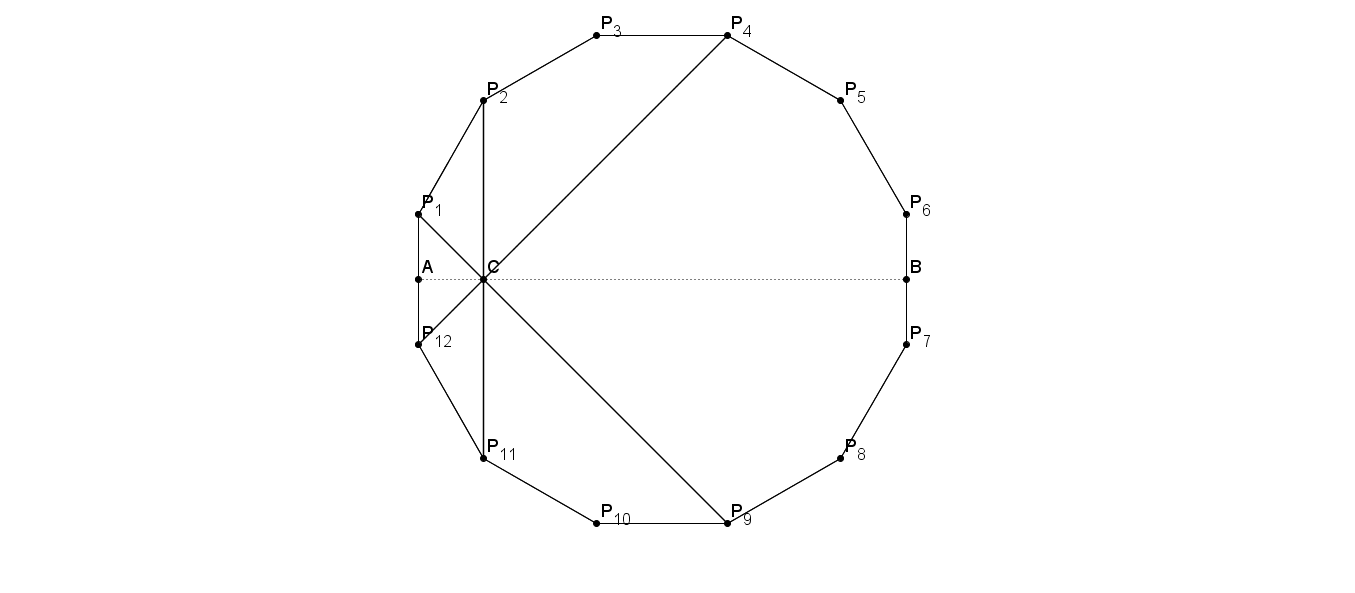
\includegraphics[width=1.2\textwidth]{./figures/chpt1/1_5_8.png}
	\caption{Exercise 1.5.8}
	\label{fig:1_5_8}
\end{figure}

\begin{Exercise}
	We see from figure~\ref{fig:1_5_8} that indeed they are concurrent, but we need to prove this rigorously.

	The angle of $CP_1P_{12} = P_{12}P_1C = 45^{\circ}$ by looking at polygons created by the diagonals itself and the dodecagon.
	If we let the side length of the dodecagon be $x$, then $P_1P_9$ and $P_4P_{12}$ intersects at exactly $x/2$ distance away from the segment $P_1P_{12}$ by the properties of right triangle ($P_1P_{12}C$ is the special right triangle).

	It is obvious that $P_2P_{11}$ creates a trapezoid with angles 150 and 30. 
	Since we have the angle, we can now find the height of the trapezoid, which is exactly $x/2$ as predicted (using $\sin 30^{\circ}$).

	One has to tie this proof a bit tighter for the Putnam exam though by proving the diagonals first intersect line $AB$,
	\footnote{a symmetry argument should do here} but
	this is a good enough sketch I think. \qed
\end{Exercise}

\begin{Exercise}
	\begin{enumerate}
		\item Average rate by definition means the total distance over total time. 
		The key point to note is that the time spent driving from point $A$ to $B$ will be \emph{more} then the other way around, 
		since the speed is slower. 
		Henyce, the average rate is less than 50 miles per hour. 

		Algebraically, let $x$ be the distance between $A$ and $B$.
		We have the following:
		\begin{align}
			s &= \frac{d}{t} \\
			&= \frac{2x}{\frac{x}{40} + \frac{x}{60}} \\
			&= \frac{2(2400)}{40 + 60}
		\end{align}
		and we see that it's the harmonic average of the two speeds. 
		The cool thing is that the distance doesn't matter at all! \qed

		\item Of course, we see physically that the two must equal, but we should do this algebraically.
		We'll do this the hard way, by keeping both the amounts of liquid and the volume of the spoon as variables (instead of scaling the spoon volume to 1).

		Let $V$ be the volume of the coffee (and the cup of cream), then let $x$ be the volume of the spoon. 
		The initial scoop will result in $V$ coffee and $x$ cream in the coffee cup and $V-x$ cream in the cream cup.
		Now the scoop from the coffee cup will contain $x \cdot \frac{x}{V+x}$  amount of cream, and $x \cdot \frac{V}{V+x}$ amount of coffee.

		This means that the final amount of cream left in the coffee cup is $x - x\cdot \frac{x}{V+x}$, while the total amount of 
		coffee in the coffee cup is $0 + x\cdot \frac{V}{V+x}$. 
		One can verify easily that they are equal. \qed

		\item Let the radius of the Earth in feet be $R$, then the original length of the rope is $2\pi R$.
		Extending that string by 6 feet will result in the new length to be $2\pi R + 6$. 

		We wish to find the new radius which have that value as its circumference; this is done by dividing by $2\pi$.
		Thus, the string is lifted by $\frac{6}{2\pi}$ total feet, which is around 1 foot and greater than an inch. \qed
	\end{enumerate}
\end{Exercise}

\end{document}
